\documentclass{article}
\usepackage{algorithm}
\usepackage{algpseudocode}
\usepackage{float}
\usepackage{hyperref}
\usepackage{graphicx}
\graphicspath{ {images/} }
\usepackage{enumerate}
\usepackage{xcolor}
\usepackage{hyperref}
\usepackage{tabu} %for longtabu
\usepackage{hhline} %for double \hline in longtabu
\usepackage{listings}
\usepackage[a4paper, total={6in, 8in}]{geometry}

\usepackage[utf8]{inputenc}
\usepackage[english]{babel}
\usepackage{amsthm}
\theoremstyle{definition}
\newtheorem{definition}{Definition}[section]

\begin{document}

\begin{titlepage}
	\newcommand{\HRule}{\rule{\linewidth}{0.5mm}}
	\center % Centre everything on the page
	\textsc{\LARGE Iowa State University}\\[1.5cm]
	\HRule\\[0.4cm]
	{\huge\bfseries R2U2 Demo (Jan.2018) Documentation}\\[0.4cm]
	\HRule\\[1.5cm]
	\vfill\vfill\vfill
	{\large\today}
	\vfill 
\end{titlepage}

\begin{titlepage}
	\newcommand{\HRule}{\rule{\linewidth}{0.5mm}}
	\center % Centre everything on the page
	\textsc{\LARGE Quick Demo Setup}\\[1.5cm]
	System input: combined sensor data in binary format\\
	System output: verdict and time stamp for each future time monitor assembly instruction
	%\HRule\\[0.4cm]
	%{\huge\bfseries R2U2 System Documentation}\\[0.4cm]
	%\HRule\\[1.5cm]
%	\vfill\vfill\vfill
%	{\large\today}
%	\vfill 
\end{titlepage}

\section{Brief Setup Process}
This section talks about how to generate required files and steps to run the demo. \\
Note: 1) The text mark with \colorbox{blue!30}{\hspace{0.5cm}} means the command typed in terminal.\\
2) The text marked in \textcolor{green!100}{green} are the files that require manually modify.
\subsection{Preprocessing}
\begin{enumerate}
\item Generate checker associated file
	\begin{enumerate}
		\item Modify \textcolor{green!100}{inputs.py} (section \ref{inputs.py}) to specify the input data format and name, then run \colorbox{blue!30}{python inputs.py }
		\item Generate \textcolor{purple!30}{at\_checkers.vhd} and \textcolor{purple!30}{log\_input\_pkg.vhd} by running \colorbox{blue!30}{python transformer.py}
		\item Write atomic assertion configuration in \textcolor{green!100}{input.ast} (section \ref{input.ast}), run \colorbox{blue!30}{python assert\_convert.py} to convert the assertion into binary configuration file named \textcolor{purple!30}{res.atc}.
	\end{enumerate}
\item Generate binary instruction assembly code and its interval file (.imem and .int)
	\begin{enumerate}
		\item write assembly code in \textcolor{green!100}{casestudy.ftasm}, run \colorbox{blue!30}{sh convert.sh} in folder
	\end{enumerate}
\item Generate UART byte data
	\begin{enumerate}
		\item Modify parameters associated with data byte size in \textcolor{green!100}{python gen\_uart\_data.py} (section \ref{gendata.py}). These parameters should be the same as \textcolor{purple!30}{R2U2\_pkg.vhd}. Run command \colorbox{blue!30}{python gen\_uart\_data.py}
	\end{enumerate}	
\end{enumerate}

\subsection{Hardware Connection}
\begin{enumerate}
	\item FPGA Board Connection
	\begin{enumerate}
		\item Connect the JTAG with PC for downloading bitfile. See Figure \ref{FPGA}.
	\end{enumerate}
	\item UART Connection
	\begin{enumerate}
		\item Connect the UART module with PC, connect UART module PIN \textbf{DIN} with Zedboard \textbf{JP4}, PIN \textbf{DOUT} with Zedboard \textbf{JP3}. See Figure \ref{uart}.
	\end{enumerate}
	\item Reset button is located in Zedboard  \textbf{BTNC(P16)}.
\end{enumerate}

\subsection{Run}
\begin{enumerate}
	\item Download bitfile into FPGA
	\item Modify \textcolor{green!100}{ser.py} (section \ref{ser.py}) to specify the correct uart port on PC and .dat byte size (should be the same size as in \textcolor{purple!30}{R2U2\_pkg.vhd}.
	\item Run  \colorbox{blue!30}{sudo python ser.py}. This script will send atomic checker's and future time monitor's configuration to the board automatically.
	\item Type binary data as input (same format as each line in \textcolor{purple!30}{logged\_data.dat}) and press enter. You will see the result displayed in the terminal window.
\end{enumerate}

\begin{figure}[h]
\caption{Zedboard connection setup}
\label{FPGA}
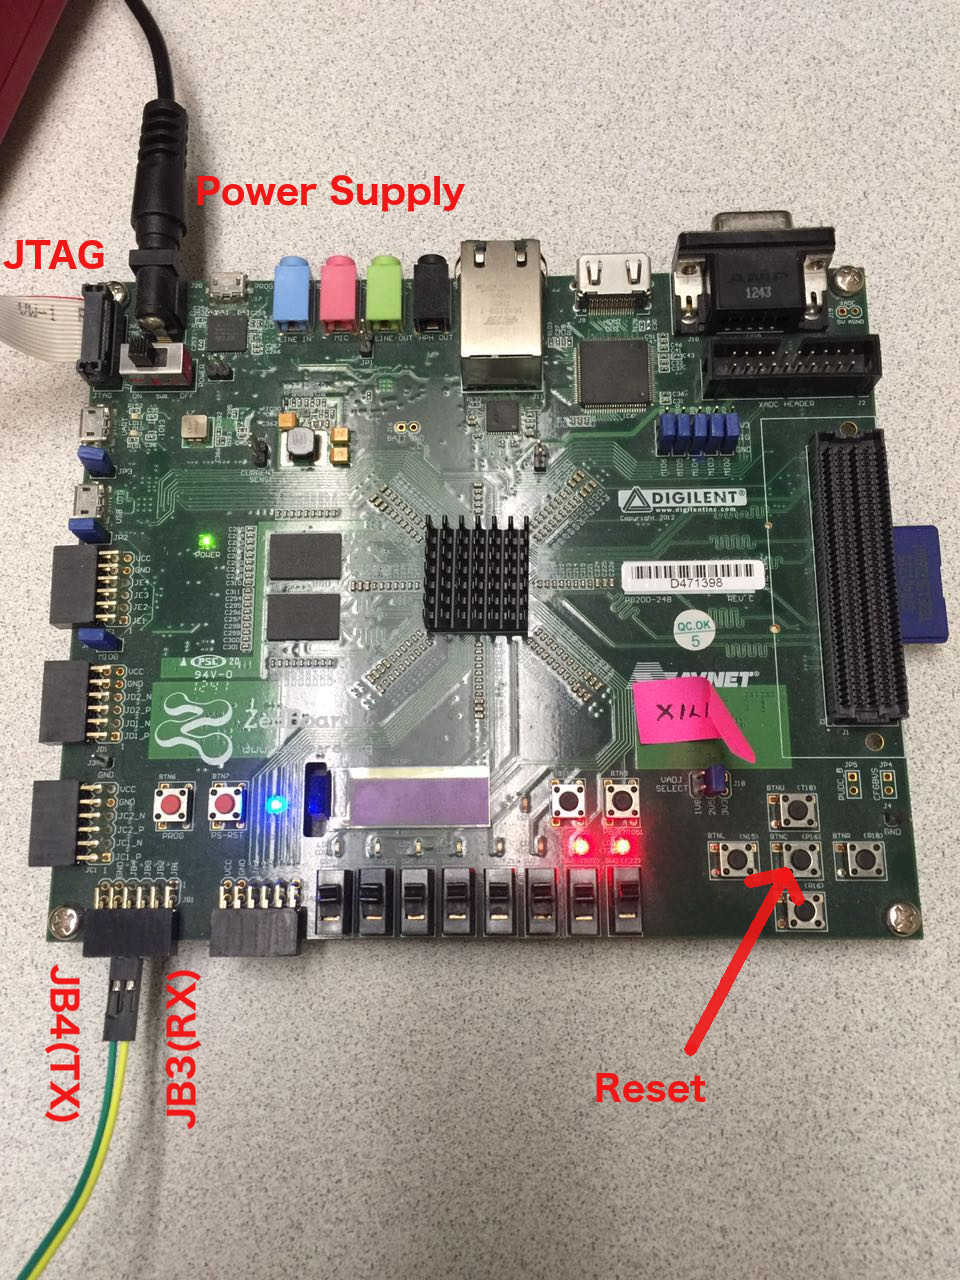
\includegraphics[width=8cm]{./fig/FPGA.jpg}
\centering
\end{figure}

\begin{figure}[h]
\caption{UART module connection setup}
\label{uart}
\includegraphics[width=8cm]{./fig/UART.jpg}
\centering
\end{figure}

\clearpage






\section{Details of Scripts and Files}
\subsection{inputs.py}\label{inputs.py}
(only compatiable with python 2.x)\\
Processing raw data file (similar to .csv) to the data format we want.\\
Parameters and functions:
\begin{enumerate}
	\item DATA\_SET: Raw data set file
	\item class subclass(CsvParser): \\
e.g.
\begin{lstlisting}[language=Python]
class Gs111m(CsvParser):
	def __init__(self):
		CsvParser.__init__(self)
		self.file = DATA_SET + "/gs111m_0.csv"
		self.addConfig(9, "float", 10, 24, "roll_angle", "in 1/2^10 rad")
		self.addConfig(8, "float", 10, 24, "pitch_angle", "in 1/2^10 rad")
\end{lstlisting}
Comment: Create a subclass. It will subtract the data you mentioned in \textbf{self.addConfig} and output the processed data into \textbf{self.file}
The self.file will look like:
\begin{center}
\begin{tabular}{ c|c} 
 \hline
 roll\_angle & pitch\_angle \\ 
 \hline
 -42 & 12 \\ 
 \hline
 -34 & 6\\ 
 \hline
 -25 & 3\\ 
 ...&...
\end{tabular}
\end{center}
$\triangleright$ self.addConfig(channel, type, comma, width, name, comment)\\
@ channel: Column of the data in the raw data file.\\
@ type: Float or not. If it's float, write "float", else leave null.\\
@ comma: Only used for floating data type. It specifies how many fraction bit in binary you want to reserve during the conversion.\\
@ width: Number of bits for this data.\\
@ name: Specify the name of the column data. This will affect the name used in the .vhd code.\\
@ comment: Add any comment in string as you want.

\item class subclass(AtChecker):\\
e.g.
\begin{lstlisting}[language=Python]
class AtCheckerConfig(AtChecker):
	def __init__(self, inputFiles):
		AtChecker.__init__(self, inputFiles)
		self.add("pitch_angle", "", 1, "", "", "", "")
		self.add("roll_angle", "", 1, "", "", "", "")
\end{lstlisting}
Comment: Create a subclass. The subclass specifies the filters, number of atomic checkers, etc.. The class will affect at\_checker.vhd\\
$\triangleright$ self.add(input1, input2, count, filter1, filter2, rate1, rate2)\\
@ input1: First input to the at\_checker\\
@ input2: Second input to the at\_checker, usually used for compare with @input1. We can leave it as a null string "".\\
@ count: How many atomic checkers you want for this signal.\\
@ filter1: Hardware filter you want to use for input1. The filter name should be the same as the hardware filter component\\
@ filter2: Hardware filter you want to use for input2.\\
@ rate1: Signal delta during each sampling clk for input1. Leave null if you want to monitor signal delta.\\
@ rate2: Signal delta during each sampling clk for input2.

\end{enumerate}


\subsection{input.ast}\label{input.ast}
Atomic assertion file. Specify the at\_checker.vhd operation mode. For details, refer to \textbf{Performance\_Aware\_Hardware\_Runtime\_Monitors.pdf}.
\\
e.g.\\
\begin{tabular}{|p{0.98\textwidth}|}
\hline
-16;0;0;+;$>$\\
1;0;0;+;$=$\\
100;0;0;+;$>$\\
\hline
\end{tabular}
\\
\begin{figure}[h]
\caption{Atomic checker block}
\label{ac}
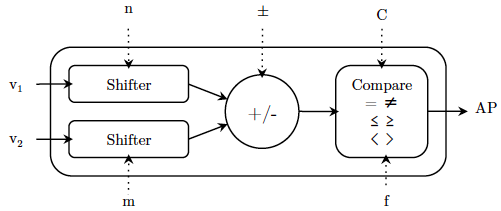
\includegraphics[width=8cm]{./fig/ast.png}
\centering
\end{figure}
Each line specifies the configuration for one atomic checker block. Consider the structure
of an atomic checker, depicted in Figure.\ref{ac}, then each line in the configuration file reads as:
C;n;m;+/-;f.

\subsection{gen\_uart\_data.py}\label{gendata.py}
Generate uart data byte by byte. Requires \textbf{.atc}, \textbf{.imem}, \textbf{.int} and \textbf{.dat} as input. I suggest leave the \textbf{.dat} file empty for the demo purpose.\\
%\begin{enumerate}
%	\item 
%	\item class subclass(CsvParser): \\
%\end{enumerate}
Parameters:\\
@ SETUP\_DATA\_WIDTH\_extend\_byte: \textbf{.atc} file configuration data width.\\
@ SETUP\_ADDR\_WIDTH\_extend\_byte: \textbf{.atc} file configuration address width.\\
@ DATA\_BYTE\_WIDTH\_extend\_byte: binary logged data bit width (each line width of \textcolor{purple!30}{logged\_data.dat}).\\
These three parameters should be the same as in \textcolor{purple!30}{R2U2\_pkg.vhd}.
 
 \subsection{ser.py}\label{ser.py}
 
 \begin{enumerate}
 	\item serial.Serial()\\
	e.g.
	\begin{lstlisting}[language=Python]
ser = serial.Serial(
    port='/dev/ttyUSB0',
    timeout=0,
    # baudrate=9600,
    # parity=serial.PARITY_ODD,
    # stopbits=serial.STOPBITS_TWO,
    # bytesize=serial.SEVENBITS
 )
	\end{lstlisting}

Comment: By default, it is 9600 baud rate 8IN1 mode. You only need to specify the PC port that the UART is connecting to.
	\item parameters:
	@ DATA\_BYTE\_WIDTH\_extend\_byte: (same as \textcolor{purple!30}{gen\_uart\_data.py})
  \end{enumerate}
 

 \section{Demo Screenshot}
 Suppose all data is preprocessed properly. How are the screenshot sample:\\
 1. Run \textcolor{purple!30}{ser.py}, it will wait for sensor input as in Figure \ref{step1}.
  \begin{figure}[h]
\caption{Wait for input}
\label{step1}
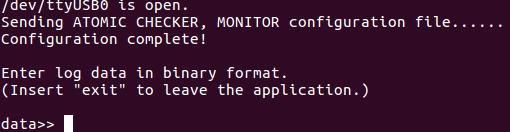
\includegraphics[width=12cm]{./fig/step1.png}
\centering
\end{figure}

2. Copy one line of data from \textcolor{purple!30}{logged\_data.dat} as sensor input:\\
\begin{figure}[h]
\caption{Output sampel}
\label{step2}
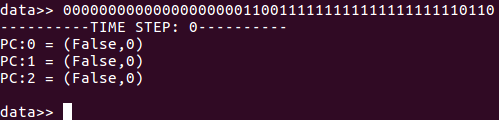
\includegraphics[width=12cm]{./fig/step2.png}
\centering
\end{figure}
The future time monitor output is shown in Figure \ref{step2}.\\

You can keep feeding sensor input and see output in each time step. 
\end{document}